% Options here are passed to the article class.
% Most common options: 10pt, 11pt, 12pt
\documentclass[10pt]{datasheet}

% Input encoding and typographical rules for English language
\usepackage[utf8]{inputenc}
\usepackage[english]{babel}
\usepackage[english]{isodate}

% tikz is used to draw images in this example, but you can
% also use \includegraphics{}.
\usepackage{graphicx}
\usepackage{float}
\usepackage{subcaption}

% These define global texts that are used in headers and titles.
\title{IM06: 8bit Disk Drive Temp Storage}
\author{disharmonica\_}
\tags{item-memory, disk-drive, temp-storage}
\date{25 December 2024}
\revision{Revision 1}
\begin{document}
\maketitle

\section{Features}
\begin{itemize}
\item{Extremely compact, 13x9x7 lwh}
\item{Very accessible inputs, output into waterstream, perfect for plumbing}
\item{Has simple temp logic that gives out both boxes, if another one was in storage already}
\item{Uses water buckets as placeholders, turns them into buckets to store very compact when not needed}
\item{Quick cycle and reset, min.102gt - max.598gt = 17.5 seconds on average per request}
\item{Only uses 21 hoppers, wiring for hopperlocking included}
\end{itemize}

\section{Applications}

\begin{itemize}
\item{Dynamic sorting partial box merging loop}
\end{itemize}

\section{General Description}
The IM06 can temporarily store and retrieve boxes with a binary code. Intended for keeping the leftover partials of bulk items, for future merging operations. 256 different types can be held by this device.

\vfill\break

\begin{figure}[H]
    \centering
    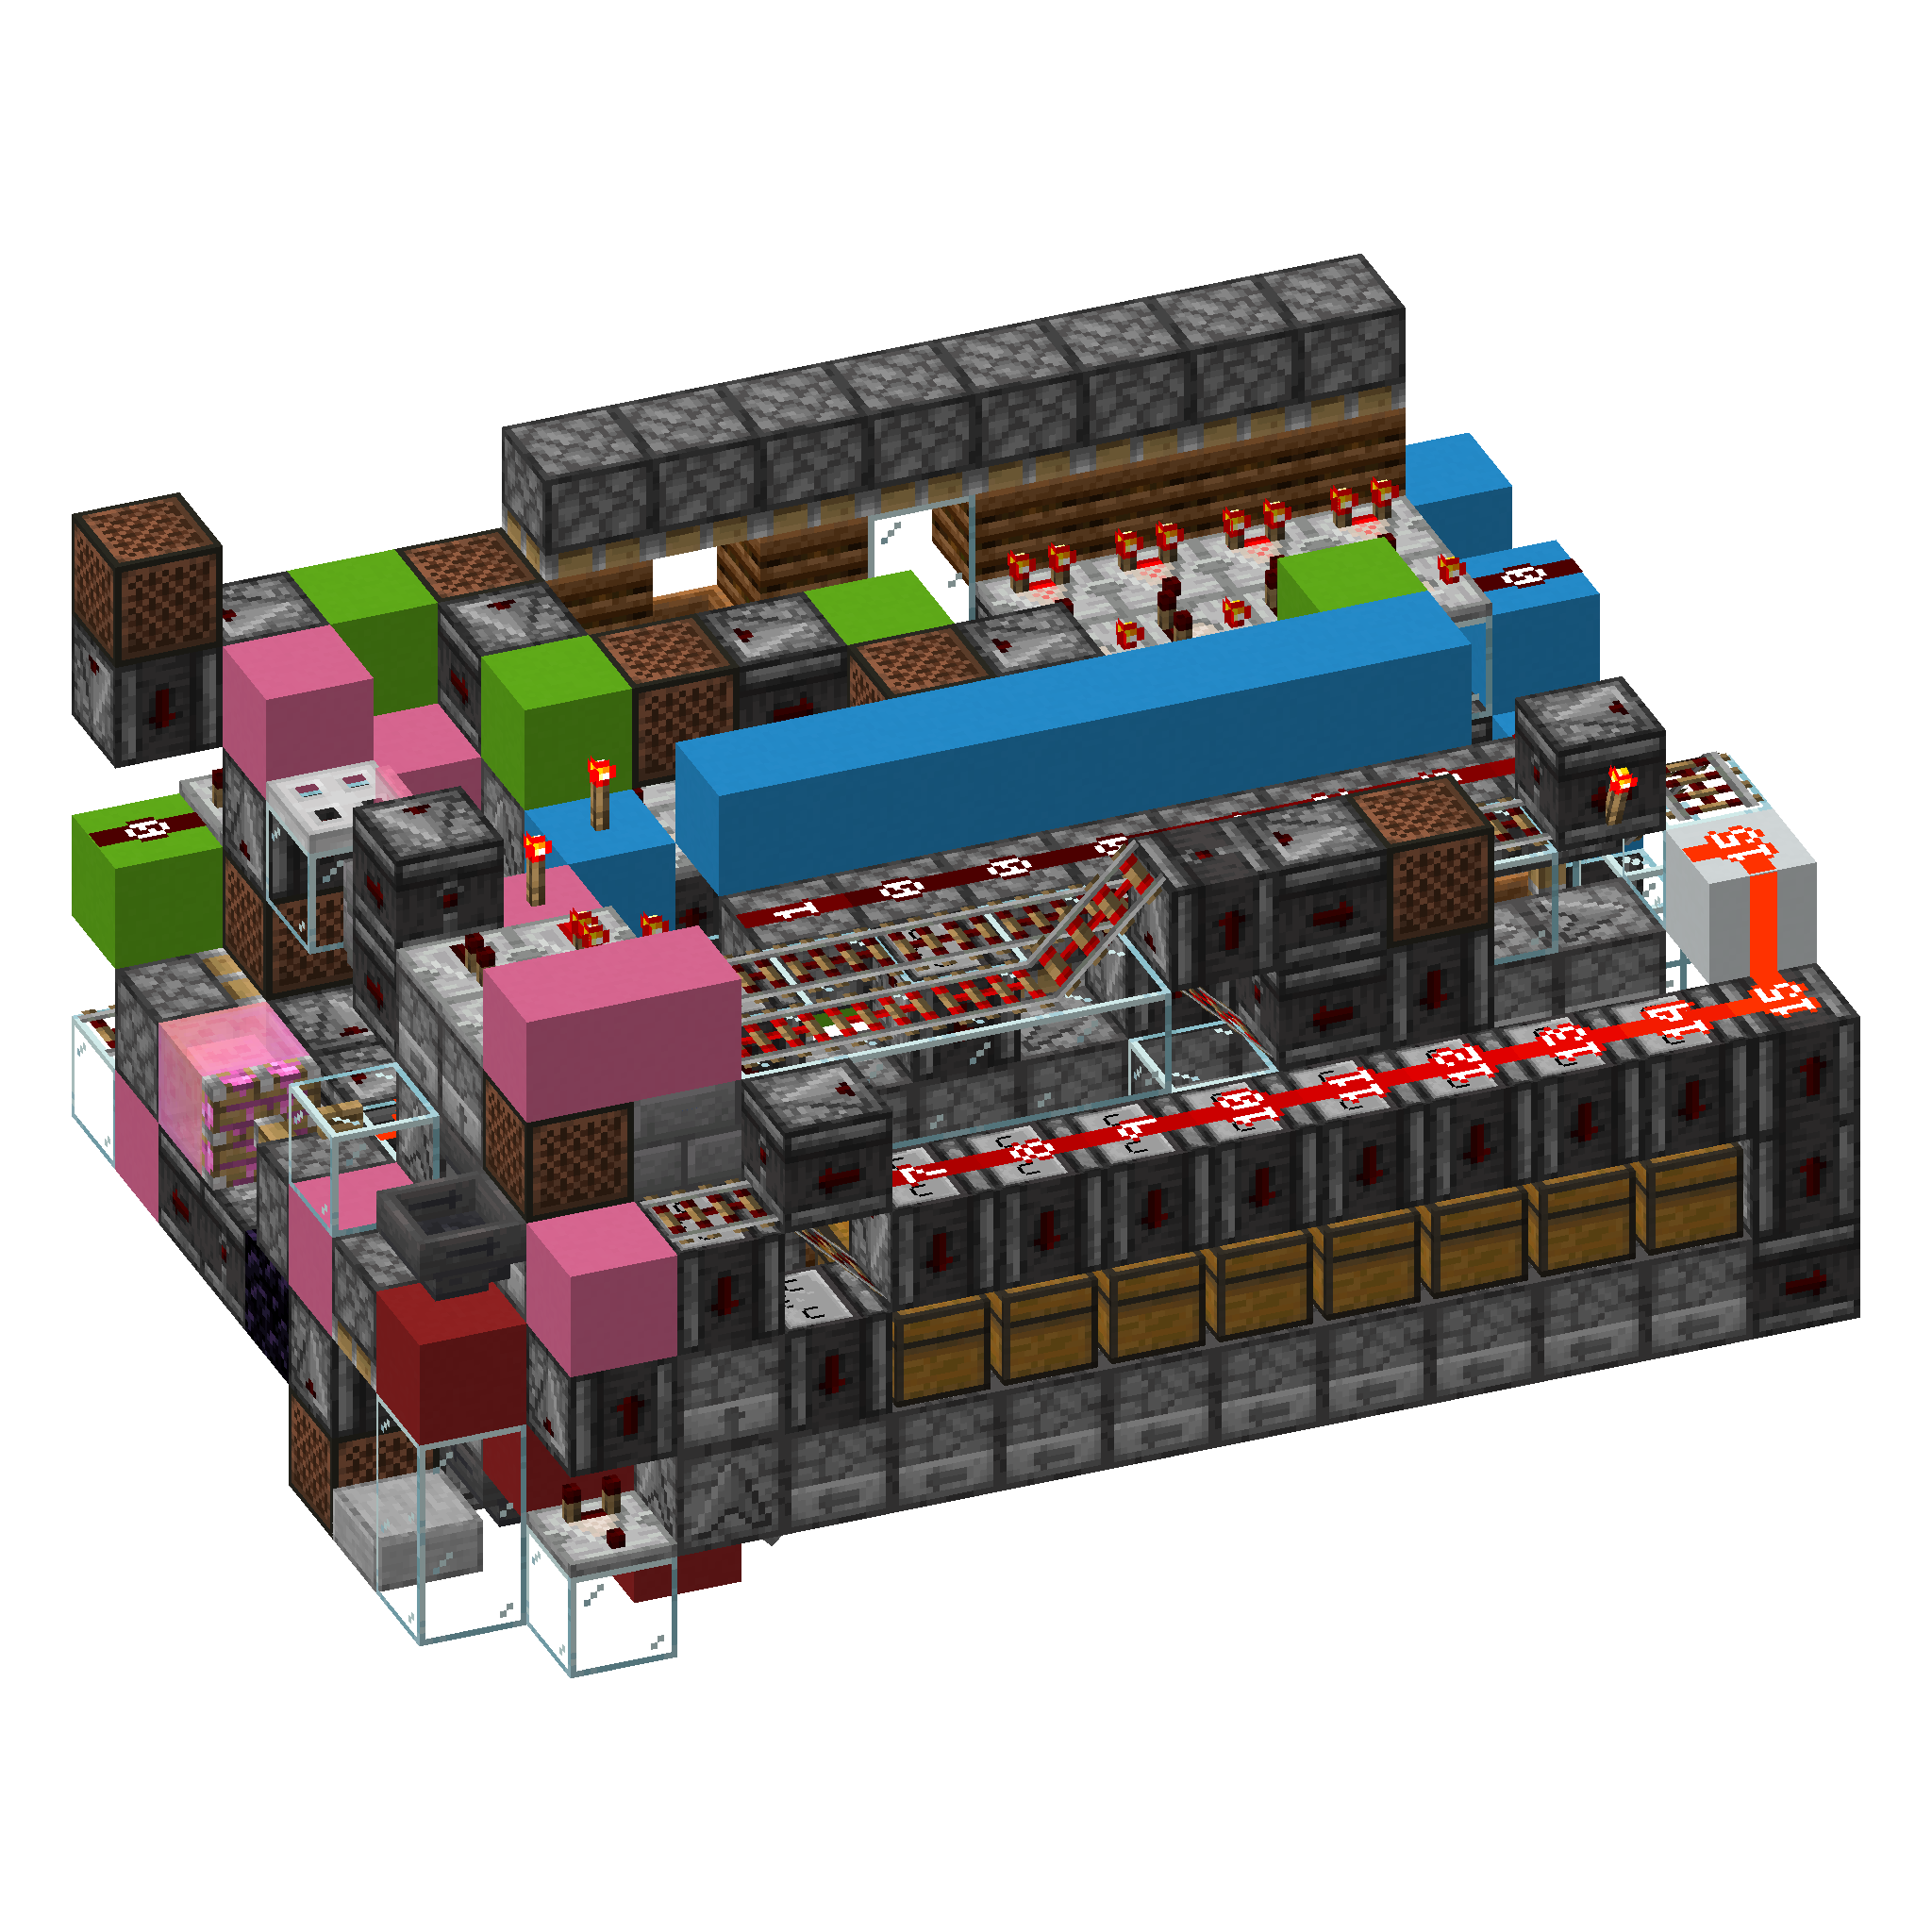
\includegraphics[width=0.48\textwidth]{area_render_35_.png}
    \caption{\centering 8bit Disk Drive Temp Storage}
\end{figure}

% For wide tables, a single column layout is better. It can be switched
% page-by-page.
\onecolumn

\section{Device Specifications}

\begin{table}[H]
    \caption{Inputs}
    \begin{tabularx}{\textwidth}{l | c | X}
        \thickhline
        \textbf{Name} & \textbf{Range} & \textbf{Description} \\
        \hline
        Address Bits 0-7 & 0-1 & Binary address of box. \\
        \hline
        Hopperlocking & 0-1 & Hopperlocking control. \\
        \hline
        Trigger & Pulse & Trigger to start the process. \\
        \hline
        Box input & box & Box input. Usually a partial box from a splitter. \\
        \thickhline
\end{tabularx}
\end{table}

\begin{table}[H]
    \caption{Outputs}
    \begin{tabularx}{\textwidth}{l | c | X}
        \thickhline
        \textbf{Name} & \textbf{Range} & \textbf{Description} \\
        \hline
        Box output & box & Box output. Outputs two boxes with the same type simultaneously when a match is found. Otherwise, the input box is stored. \\
        \thickhline
\end{tabularx}
\end{table}

\begin{table}[H]
    \caption{Device Specifications}
    \begin{tabularx}{\textwidth}{l | c c c | c | X}
        \thickhline
        \textbf{Parameter} & \textbf{Min.} & \textbf{Typ.} & \textbf{Max.} &
        \textbf{Unit} & \textbf{Conditions} \\
        \hline
        Minimum Latency & 102 & - & 598 & gt & From input to pair output \\
        \hline
        MC Version & 1.17 & 1.19.3 & - & MCV & Latest version at time of writing: 1.21.4\\
        \hline
        Dimensions & & 13 x 9 x 7 & & Blocks & \\
        \thickhline
\end{tabularx}
\end{table}

\section{Testing Data}
\begin{table}[H]
\caption{Executed Tests}
\begin{tabularx}{\textwidth}{l | X}
    \thickhline
    \textbf{Test} & \textbf{Result} \\
    \hline
    Pair generation test & Device was able to produce pairs corresponding to the address. \\
    \thickhline
\end{tabularx}
\end{table}

\section{Download Information}
\begin{table}[H]
    \caption{Download Information}
    \begin{tabularx}{\textwidth}{l | l | l | X}
        \thickhline
        \textbf{Identifier} & \textbf{MC} & \textbf{File} & \textbf{Description} \\
        \hline
        IM06 & 1.20.1 & \href{https://github.com/Soontech-Annals/Archive/blob/8413f90a054b6c415703bae02badeba7541344f6/Archive/item-memory/IM06\%208bit\%20Disk\%20Drive\%20Temp\%20Storage/IM06\_8bit\_Disk\_Drive\_Temp\_Storage.litematic?raw=1}{IM06\_8bit\_Disk\_Drive\_Temp\_Storage.litematic} & Schematic of device. \\
        \hline
        \thickhline
    \end{tabularx}
\end{table}

\end{document}

